%=========================================================

% Here you can choose to compile with or without solutions.
% However, this definition is ignored if you use any
% command from the `Makefile`.
\providecommand{\withSol}{\iftrue}

%=========================================================

\documentclass
[twoside,german,colorbacktitle,accentcolor=tud9c]
{tudexercise}

\usepackage[T1]{fontenc}
\usepackage[utf8]{inputenc}
\usepackage[ngerman]{babel}
\usepackage{amstext}
\usepackage{amsmath}
\usepackage{graphicx}
%\usepackage{setspace}
\usepackage{multicol}
\usepackage{mathtools}
\usepackage{dsfont}
\usepackage{units}
%\usepackage{subfigure}
\usepackage{color}
\usepackage{booktabs}
\usepackage{fancyref}
\usepackage{gensymb}
\usepackage{tikz}
\usetikzlibrary{shapes.misc} 
\usepackage[verbose]{placeins}%Floatbarrier
\tikzset{root/.style={align=center,draw=none},level 2/.style={align=center,left=1.5cm}}


%=========================================================


\setcounter{section}{3}
%=========================================================

\newcommand{\grp}{F}

%=========================================================


\begin{document}

\title{GDV 2 -- Theorie Übung \arabic{section}}
\subtitle{Sommer Semester 2019}
\subsubtitle{Übungsgruppe \grp{}}

\maketitle

%=========================================================



\begin{examheader}
	\textmb{GDV 1 - Theorie Übung \arabic{section} | Gruppe \grp{}}\\
	\begin{tabular}{l l l l l}
		Moritz Fuchs	& Alexander Jäger	& Amon Ditzinger	& John Kalkhof	\\
	\end{tabular}
\end{examheader} 


%=========================================================
% Anpassung an Aufgabenstellung
\renewcommand\thesubsection{Aufgabe \arabic{subsection}}
\renewcommand\thesubsubsection{\alph{subsubsection})}

%=========================================================
\FloatBarrier
\newif\ifvimbug
\vimbugfalse

\ifvimbug
\begin{document}
\fi


\subsection{Kubische B-Splines und de Boor Algorithmus (6 Punkte)}
\subsubsection{3 Punkte}
\subsubsection{3 Punkte}

\FloatBarrier
\newif\ifvimbug
\vimbugfalse

\ifvimbug
\begin{document}
\fi


\subsection{Bernstein-Bézier-Tensorprodukte (7 Punkte)}
\subsubsection{3 Punkte}
Wir wenden de Casteljau an mit $v=\frac{3}{4}$ und $\lambda= \frac{1}{4}$:\\
\begin{tikzpicture}[grow=left,
level 1/.style={sibling distance=15mm},edge from parent/.style={-,draw},>=latex, level 3/.style={edge from child/.style={->,draw},sibling distance=15mm}]

\node[root] {$\begin{pmatrix}-2.125\\ 2.5625\\5.4375\end{pmatrix}$}
     child {node[level 2] (c1) {$\begin{pmatrix}-1\\2\\3\end{pmatrix}$}
           child {node[level 2] (c11) {$\begin{pmatrix}-1\\2\\0\end{pmatrix}$}}
       child {node[level 2] (c21) {}}
       }
 child {node[level 2] (c2) {$\begin{pmatrix}-2.5\\2.75\\6.25\end{pmatrix}$}
	child {node[level 2] (c21) {$\begin{pmatrix}-1\\2\\4\end{pmatrix}$}}
       child {node[level 2] (c22) {$\begin{pmatrix}-3\\3\\7\end{pmatrix}$}}
       };
       \draw[-, draw] (c21) -- (c2);
\end{tikzpicture}\\

\begin{tikzpicture}[grow=left,
level 1/.style={sibling distance=15mm},edge from parent/.style={-,draw},>=latex, level 3/.style={edge from child/.style={->,draw},sibling distance=15mm}]

\node[root] {$\begin{pmatrix}3\\3.4375\\4.875 \end{pmatrix}$}
     child {node[level 2] (c1) {$\begin{pmatrix}3\\2.5\\3 \end{pmatrix}$}
           child {node[level 2] (c11) {$\begin{pmatrix}3\\1\\0\end{pmatrix}$}}
       child {node[level 2] (c21) {}}
       }
 child {node[level 2] (c2) {$\begin{pmatrix}3\\3.75\\5.5 \end{pmatrix}$}
	child {node[level 2] (c21) {$\begin{pmatrix}3\\3\\4\end{pmatrix}$}}
       child {node[level 2] (c22) {$\begin{pmatrix}3\\4\\6\end{pmatrix}$}}
       };
       \draw[-, draw] (c21) -- (c2);
\end{tikzpicture}\\

\begin{tikzpicture}[grow=left,
level 1/.style={sibling distance=15mm},edge from parent/.style={-,draw},>=latex, level 3/.style={edge from child/.style={->,draw},sibling distance=15mm}]

\node[root] {$\begin{pmatrix}6.5\\1.375\\6.5625 \end{pmatrix}$}
     child {node[level 2] (c1) {$\begin{pmatrix}7.25\\1.75\\3\end{pmatrix}$}
           child {node[level 2] (c11) {$\begin{pmatrix}8\\1\\0\end{pmatrix}$}}
       child {node[level 2] (c21) {}}
       }
 child {node[level 2] (c2) {$\begin{pmatrix}6.25\\1.25\\7.75\end{pmatrix}$}
	child {node[level 2] (c21) {$\begin{pmatrix}7\\2\\4\end{pmatrix}$}}
       child {node[level 2] (c22) {$\begin{pmatrix}6\\1\\9\end{pmatrix}$}}
       };
       \draw[-, draw] (c21) -- (c2);
\end{tikzpicture}\\
Wir wenden de Casteljau an mit $u=\frac{1}{4}$ und $\lambda= \frac{3}{4}$:\\
\begin{tikzpicture}[grow=left,
level 1/.style={sibling distance=15mm},edge from parent/.style={-,draw},>=latex, level 3/.style={edge from child/.style={->,draw},sibling distance=15mm}]

\node[root] {$\begin{pmatrix}0.3359375\\2.81640625\\5.296875   \end{pmatrix}$}
     child {node[level 2] (c1) {$\begin{pmatrix}-0.84375\\2.78125\\5.296875\end{pmatrix}$}
           child {node[level 2] (c11) {$\begin{pmatrix}-2.125\\ 2.5625\\5.4375\end{pmatrix}$}}
       child {node[level 2] (c21) {}}
       }
 child {node[level 2] (c2) {$\begin{pmatrix}3.875\\2.921875\\5.296875\end{pmatrix}$}
	child {node[level 2] (c21) {$\begin{pmatrix}3\\3.4375\\4.875\end{pmatrix}$}}
       child {node[level 2] (c22) {$\begin{pmatrix}6.5\\1.375\\6.5625 \end{pmatrix}$}}
       };
       \draw[-, draw] (c21) -- (c2);
\end{tikzpicture}\\
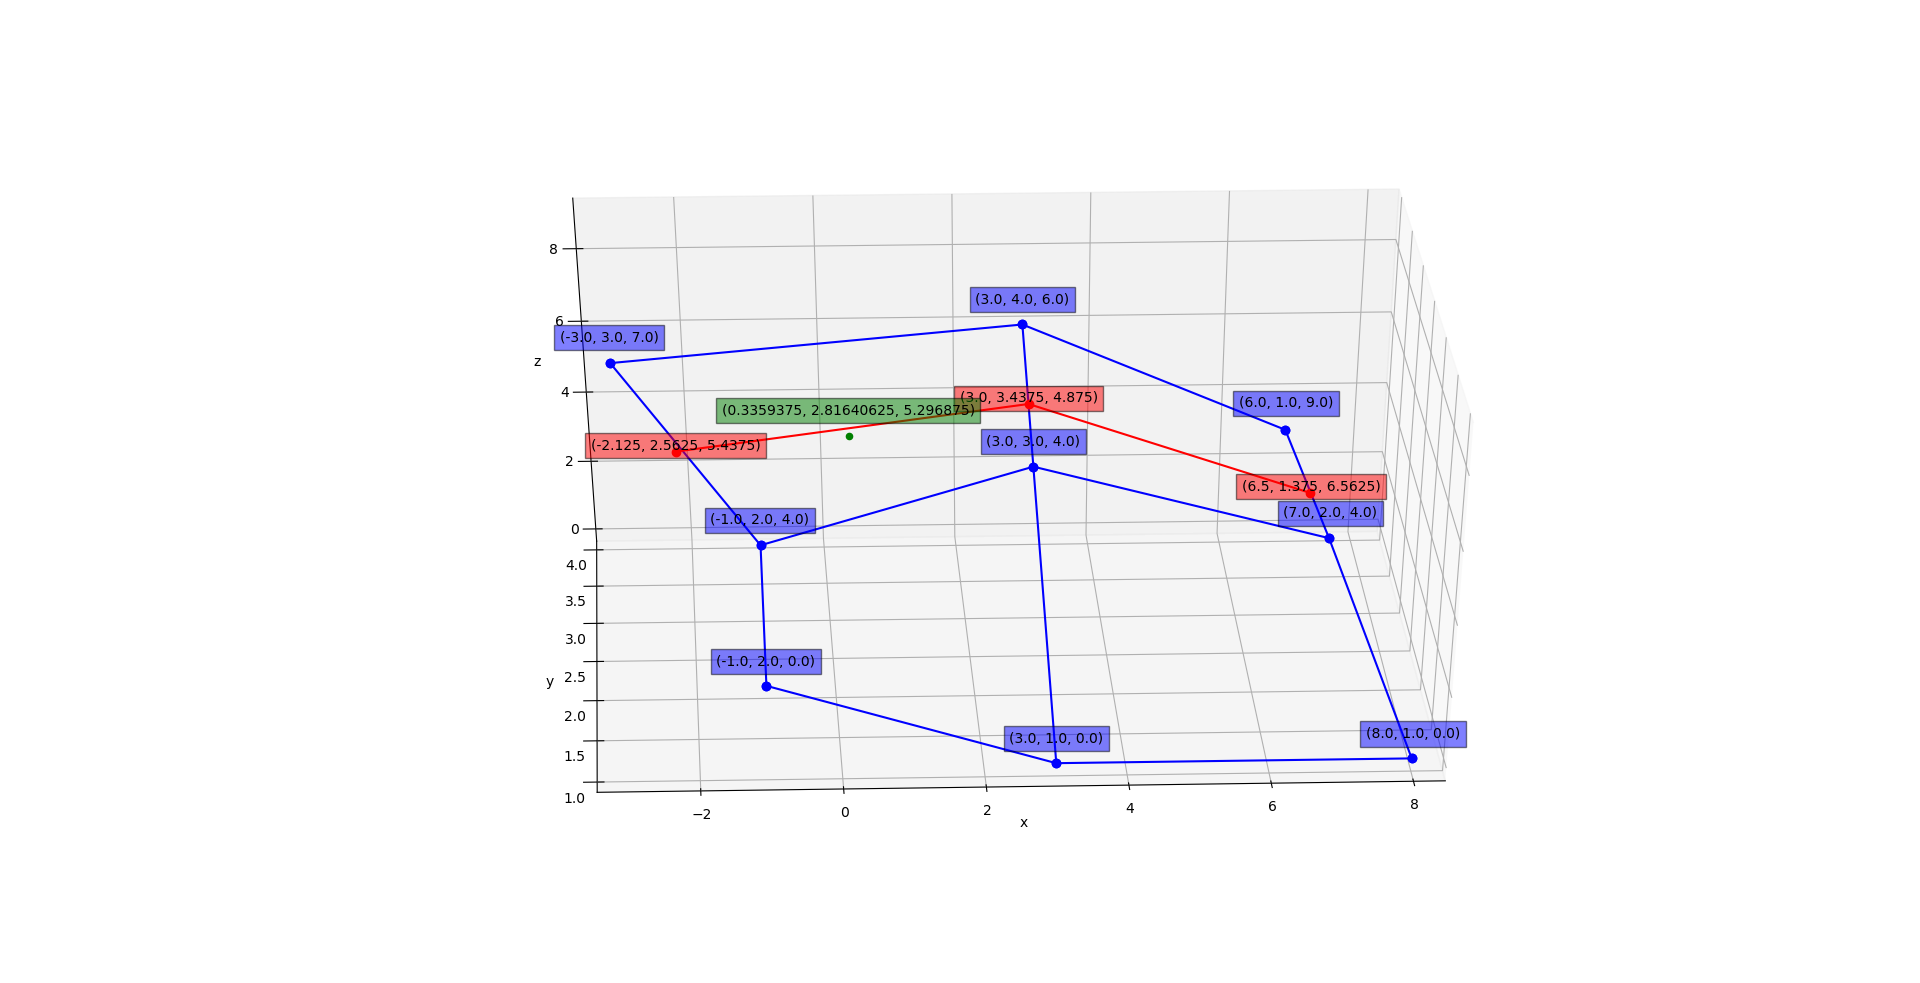
\includegraphics[width=0.9\textwidth]{2_a.png}
\subsubsection{2 Punkte}
hierzu bestimmen wir die kontrollpunkte an den Intervallsgrenzen, wie in Aufgabeteil a. in der grafik sind ist die Neue untereilung eingezeichnet.\\ 
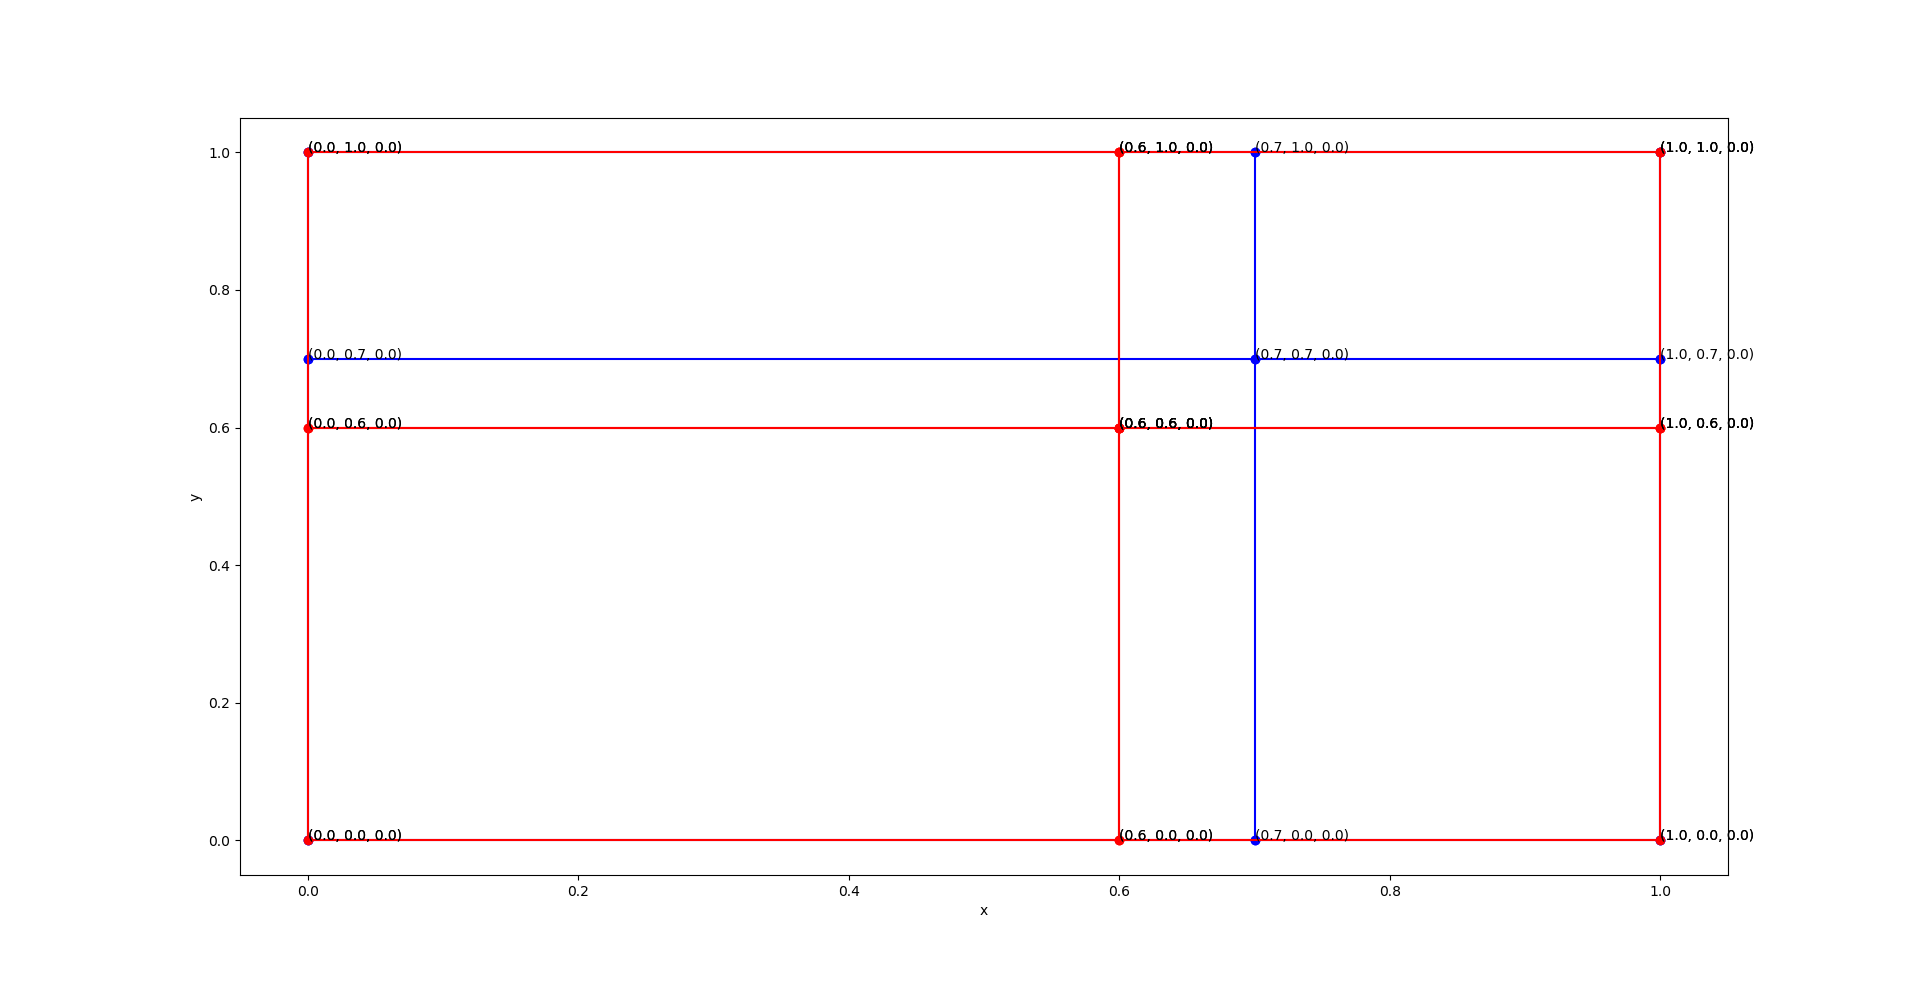
\includegraphics[width=0.9\textwidth]{2_b.png}
\subsubsection{2 Punkte}
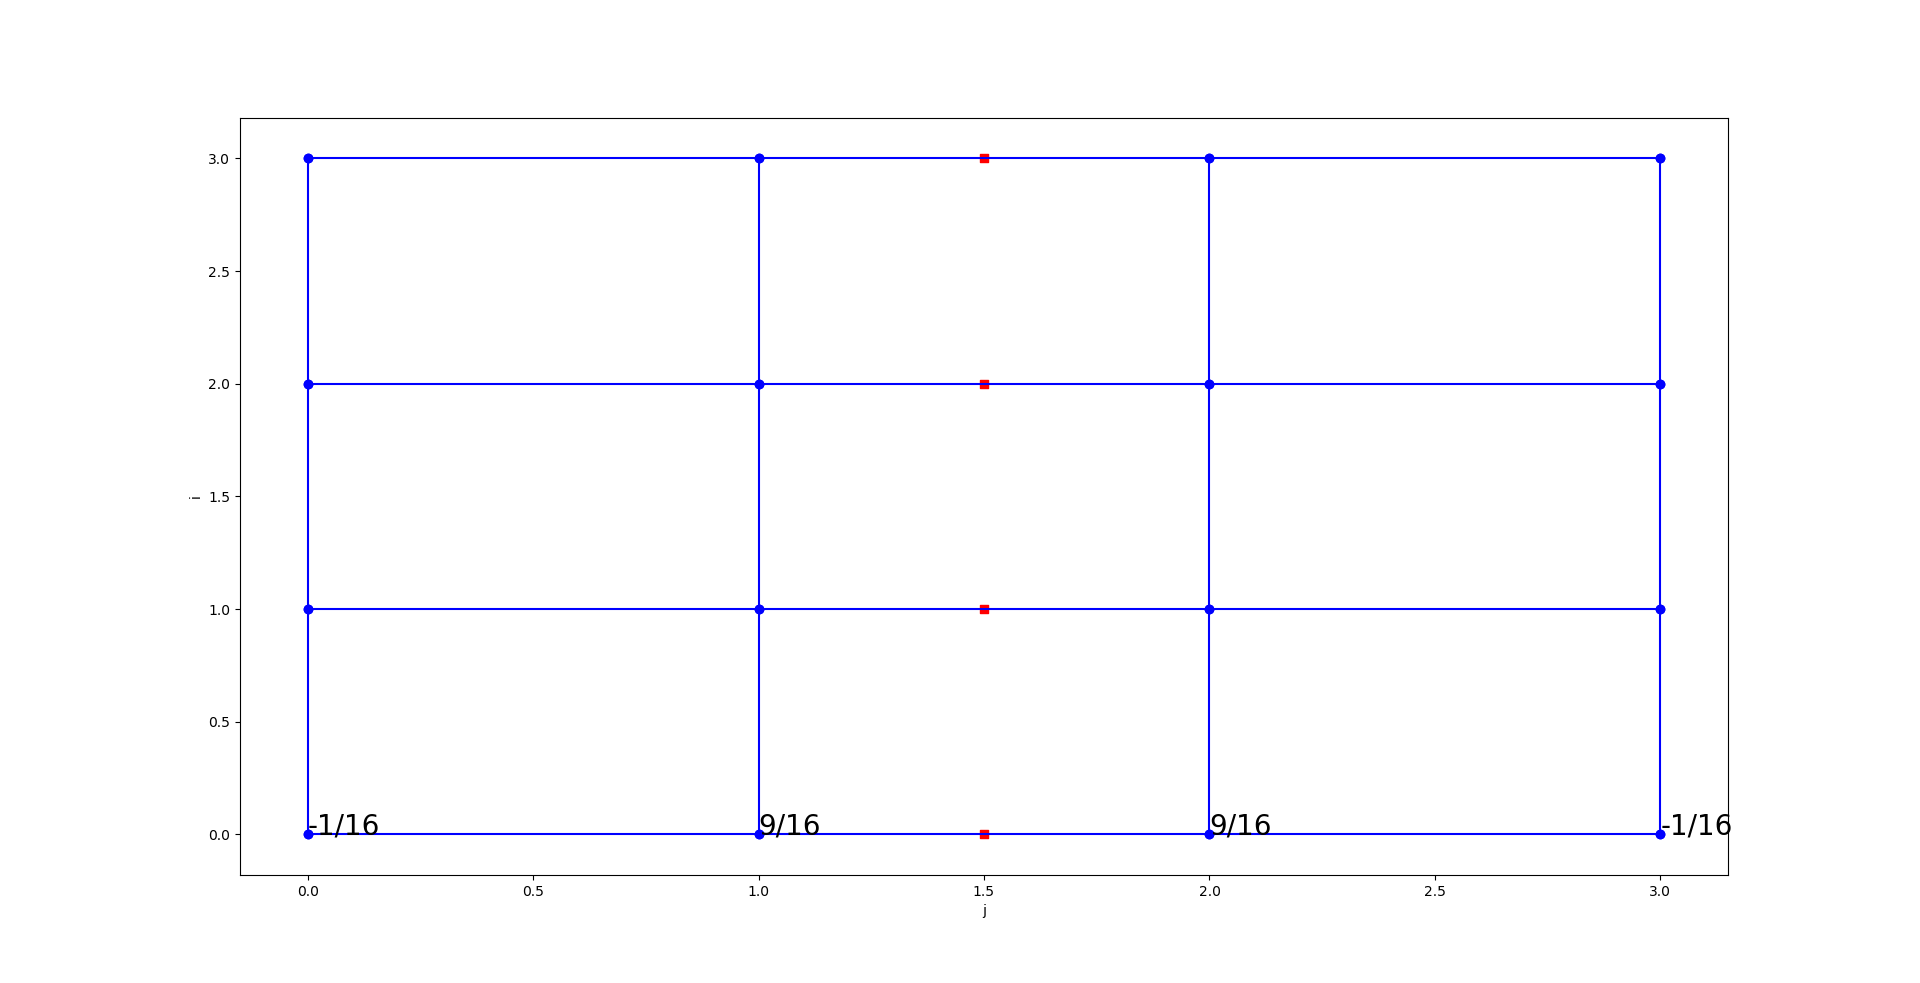
\includegraphics[width=0.5\textwidth]{2_c_P1.png}\\
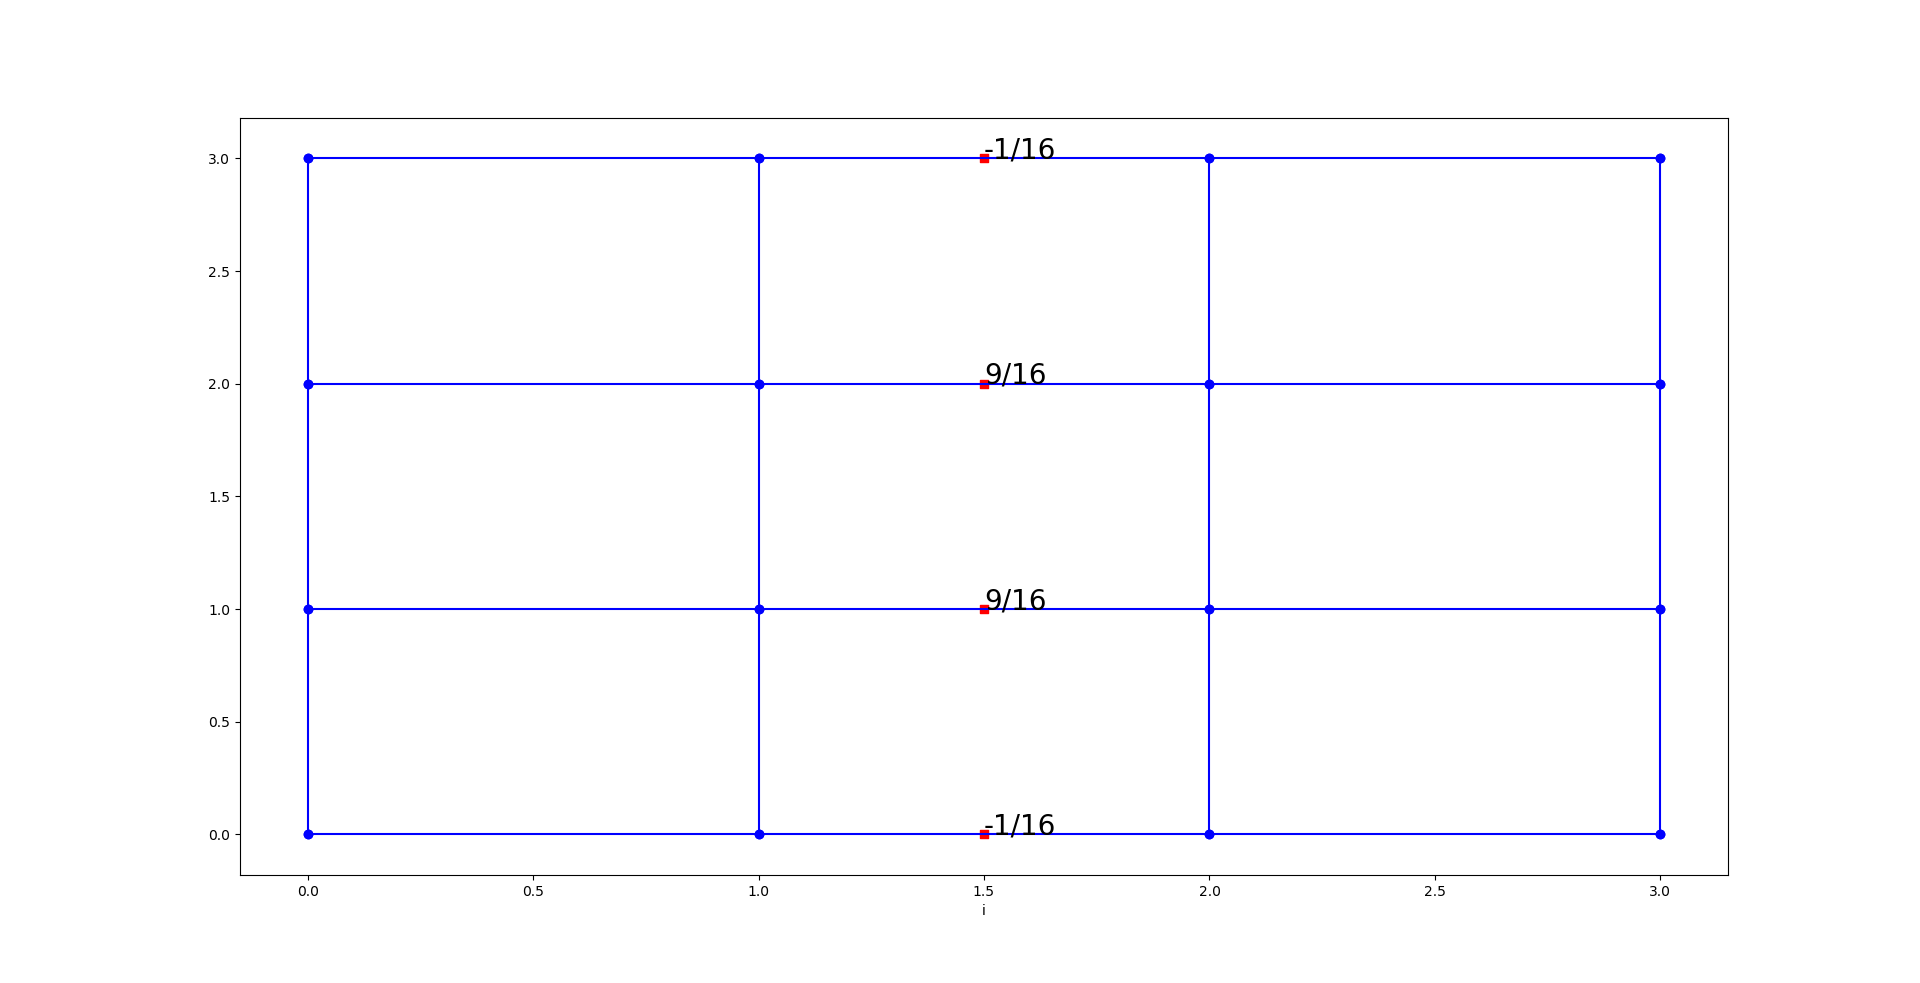
\includegraphics[width=0.5\textwidth]{2_c_P2.png}\\
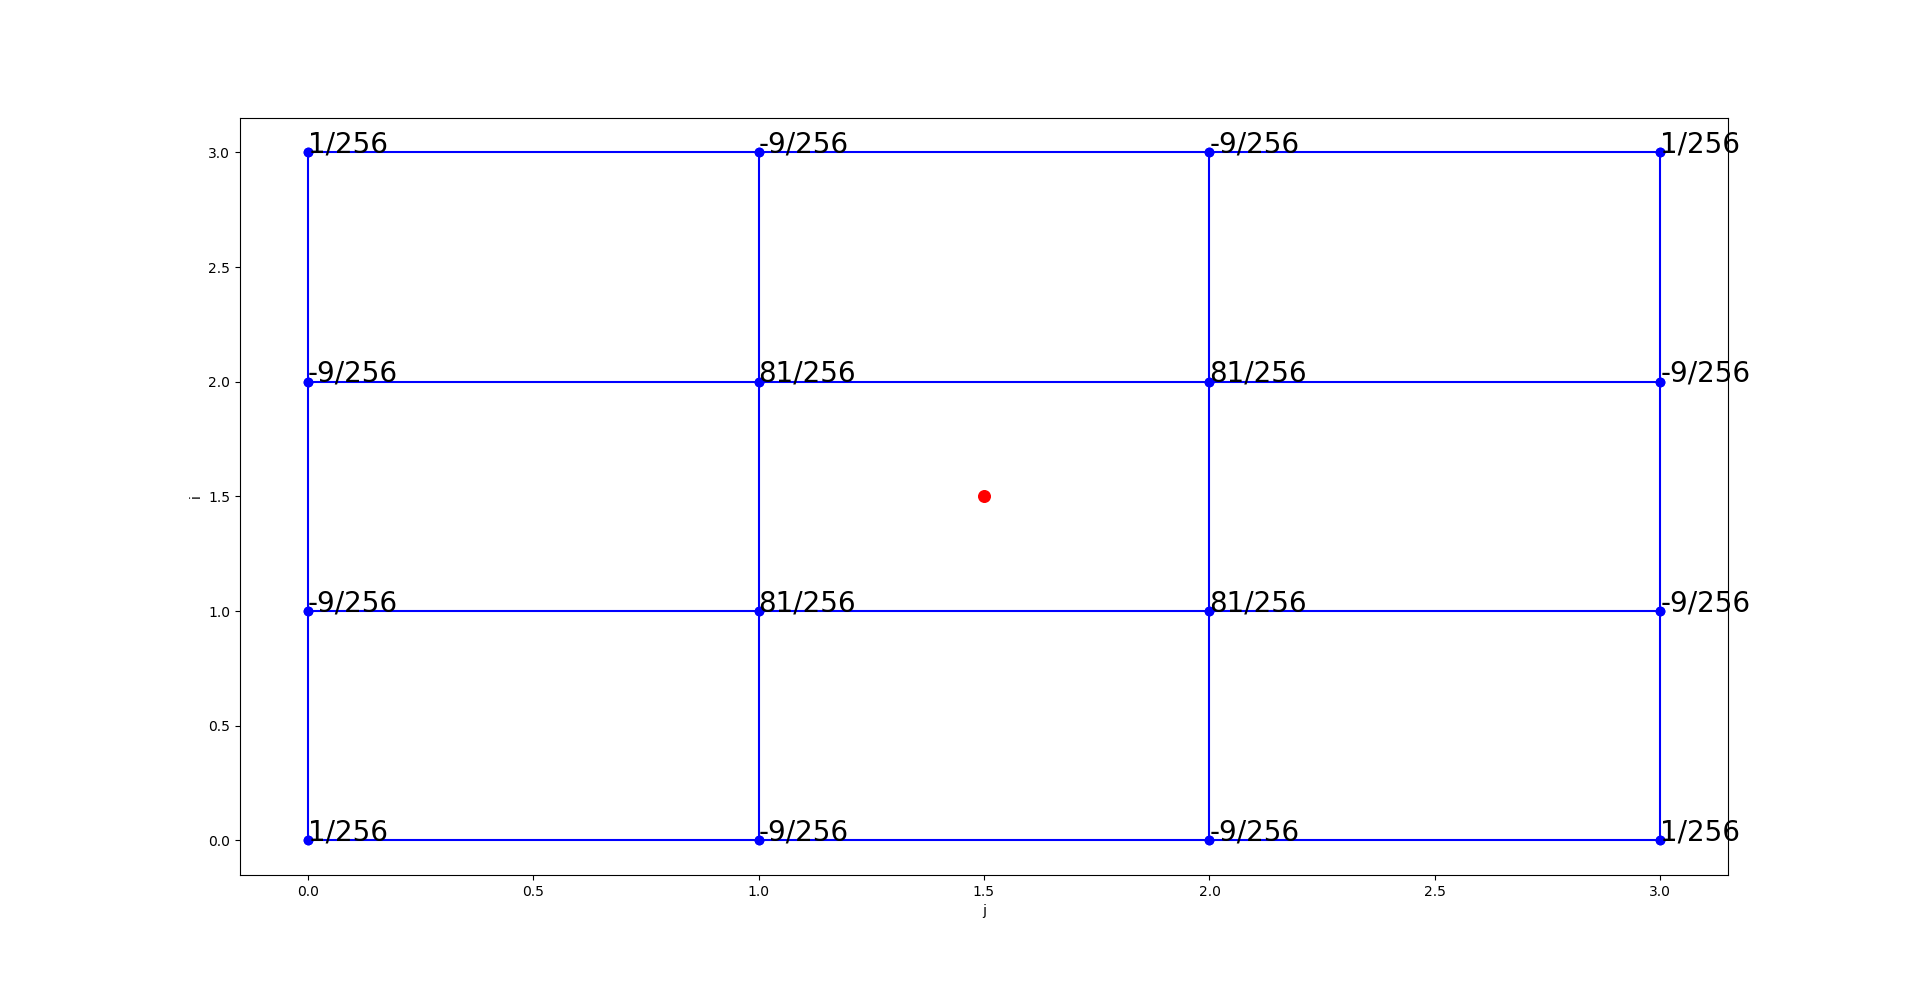
\includegraphics[width=0.5\textwidth]{2_c_P3.png}

\FloatBarrier
\newif\ifvimbug
\vimbugfalse

\ifvimbug
\begin{document}
\fi


\subsection{Implizite Oberflächen (7 Punkte)}
\subsubsection{3 Punkte}

\subsubsection{2 Punkte}

\subsubsection{2 Punkte}


%=========================================================

\end{document}
